\begin{applicationActivities}

\begin{activity}{5}
  An invertible matrix \(M\) and its inverse \(M^{-1}\) are given below:
 
  \[
    M=\begin{bmatrix}1&2\\3&4\end{bmatrix}
  \hspace{2em}
    M^{-1}=\begin{bmatrix}-2&1\\3/2&-1/2\end{bmatrix}
  \]

\vspace{1em}

  Compute \(\det(M)\) and \(\det(M^{-1})\)
  using the formula
\[
  \det\begin{bmatrix}a & b \\ c & d\end{bmatrix}=ad-bc
\]
\end{activity}

\begin{fact}
  \begin{itemize}
\item   For every invertible matrix \(M\),
  \[
    \det(M)\det(M^{-1})= \det(I)=1
  \]
  so \(\det(M^{-1})=\frac{1}{\det(M)}\).

\item  Furthermore,
  a square matrix \(M\) is invertible if and only if \(\det(M)\not=0\).
  \end{itemize}
\end{fact}

\begin{observation}
Consider the linear transformation \(A : \IR^2 \rightarrow \IR^2\) 
given by the matrix \(A = \begin{bmatrix} 2 & 2 \\ 0 & 3 \end{bmatrix}\).

\begin{center}
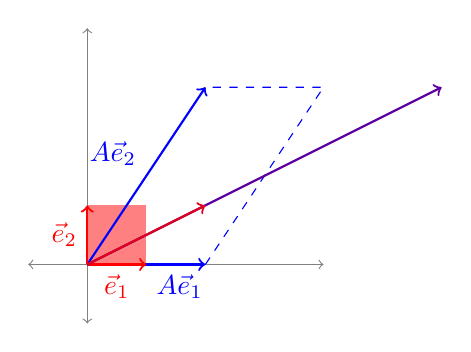
\begin{tikzpicture}[scale=0.75]
\fill[red!50] (0,0) rectangle (1,1);
\draw[thin,gray,<->] (-1,0)-- (4,0);
\draw[thin,gray,<->] (0,-1)-- (0,4);
\draw[thick,blue,->] (0,0) -- node[below right] {$A \vec{e}_1$}++ (2,0);
\draw[thick,red,->] (0,0) -- node[below] {$\vec{e}_1$}++ (1,0);
\draw[thick,blue,->] (0,0) -- node[above left] {$A \vec{e}_2$}++(2,3);
\draw[thick,red,->] (0,0) -- node[left] {$\vec{e}_2$}++ (0,1);
\draw[blue,dashed] (2,0) -- (4,3) -- (2,3);
\draw[purple!50!blue,thick,->] (0,0) -- (6,3);
\draw[purple!50!red,thick,->] (0,0) -- (2,1);
\end{tikzpicture}
\end{center}
It is easy to see geometrically that
\[
  A\begin{bmatrix}1 \\ 0 \end{bmatrix} = 
  \begin{bmatrix} 2 & 2 \\ 0 & 3 \end{bmatrix}\begin{bmatrix}1 \\ 0 \end{bmatrix}=
  \begin{bmatrix}2 \\ 0 \end{bmatrix}= 
  2 \begin{bmatrix}1 \\ 0 \end{bmatrix}
\]

It is less obvious (but easily checked once you find it) that
\[
  A\begin{bmatrix} 2 \\ 1 \end{bmatrix} = 
  \begin{bmatrix} 2 & 2 \\ 0 & 3 \end{bmatrix}\begin{bmatrix}2 \\ 1 \end{bmatrix}=
  \begin{bmatrix} 6 \\ 3 \end{bmatrix} = 
  3\begin{bmatrix} 2 \\ 1 \end{bmatrix}
\]
\end{observation}

\begin{definition}
Let $A \in M_{n,n}$.
An \term{eigenvector} for \(A\) 
is a vector $\vec{x} \in \IR^n$ such that $A\vec{x}$ is parallel to $\vec{x}$.

\begin{center}
\begin{tikzpicture}[scale=0.75]
\fill[gray!50] (0,0) rectangle (1,1);
\draw[thin,gray,<->] (-1,0)-- (4,0);
\draw[thin,gray,<->] (0,-1)-- (0,4);
\draw[thick,blue,->] (0,0) -- node[below right] {$A \vec{e}_1=2\vec e_1$}++ (2,0);
\draw[thick,red,->] (0,0) -- node[below] {$\vec{e}_1$}++ (1,0);
\draw[thick,gray,->] (0,0) -- node[above left] {$A \vec{e}_2$}++(2,3);
\draw[thick,gray,->] (0,0) -- node[left] {$\vec{e}_2$}++ (0,1);
\draw[gray,dashed] (2,0) -- (4,3) -- (2,3);
\draw[purple!50!blue,thick,->] (0,0) -- (6,3) 
  node [below right] {\(
   A\begin{bmatrix}2\\1\end{bmatrix}
     =
   3\begin{bmatrix}2\\1\end{bmatrix}
  \)};
\draw[purple!50!red,thick,->] (0,0) -- (2,1)
  node [above] {\(\begin{bmatrix}2\\1\end{bmatrix}\)};
\end{tikzpicture}
\end{center}

In other words, $A\vec{x}=\lambda \vec{x}$ for some scalar $\lambda$. 
If \(\vec x\not=\vec 0\), then we say \(\vec x\) is a \term{nontrivial eigenvector}
and we call this \(\lambda\) an \term{eigenvalue} of \(A\).
\end{definition}

\begin{activity}{5}
Finding the eigenvalues \(\lambda\) that satisfy
\[
  A\vec x=\lambda\vec x=\lambda(I\vec x)=(\lambda I)\vec x
\]
for some nontrivial eigenvector \(\vec x\) is equivalent to finding 
nonzero solutions for the matrix equation
\[
  A\vec x-(\lambda I)\vec x =\vec 0
.\]
Which of the following must be true for any eigenvalue?
\begin{enumerate}[(a)]
\item The kernel of the transformation with standard matrix \(A-\lambda I\)
must contain the zero vector, so \(A-\lambda I\) is invertible.
\item The kernel of the transformation with standard matrix \(A-\lambda I\)
must contain a nonzero vector, so \(A-\lambda I\) is not invertible.
\item The image of the transformation with standard matrix \(A-\lambda I\)
must contain the zero vector, so \(A-\lambda I\) is invertible.
\item The image of the transformation with standard matrix \(A-\lambda I\)
must contain a nonzero vector, so \(A-\lambda I\) is invertible.
\end{enumerate}
\end{activity}

\begin{fact}
  The eigenvalues \(\lambda\) for a matrix \(A\) are the values
  that make \(A-\lambda I\) non-invertible.

  \vspace{1em}

  Thus the eigenvalues \(\lambda\) for a matrix \(A\)
  are the solutions to
  the equation \[\det(A-\lambda I)=0.\]
\end{fact}

\begin{definition}
The expression \(\det(A-\lambda I)\) is called
\term{characteristic polynomial} of \(A\). \\

\vspace{1em} 

For example, when
\(A=\begin{bmatrix}1 & 2 \\ 3 & 4\end{bmatrix}\), we have

\[
  A-\lambda I=
  \begin{bmatrix}1 & 2 \\ 3 & 4\end{bmatrix}-
  \begin{bmatrix}\lambda & 0 \\ 0 & \lambda\end{bmatrix}=
  \begin{bmatrix}1-\lambda & 2 \\ 3 & 4-\lambda\end{bmatrix}
\]

\ \\
Thus the characteristic polynomial of \(A\) is
\[
  \det\begin{bmatrix}1-\lambda & 2 \\ 3 & 4-\lambda\end{bmatrix}
=
  (1-\lambda)(4-\lambda)-(2)(3)
=
  \lambda^2-5\lambda-2
\]
and its eigenvalues are the solutions to \(\lambda^2-5\lambda-2=0\).
\end{definition}

\begin{activity}{10}
  Compute $\det(A-\lambda I)$ to find the characteristic polynomial of
  $A=\begin{bmatrix} 6 & -2 & 1 \\ 17 & -5 & 5 \\ -4 & 2 & 1 \end{bmatrix}$.
\end{activity}

\begin{activity}{10}
Let $A = \begin{bmatrix} 5 & 2 \\ -3 & -2 \end{bmatrix}$.
\begin{subactivity}
Compute $\det (A-\lambda I)$ to determine the characteristic polynomial of $A$.
\end{subactivity}
\begin{subactivity}
Factor this characteristic polynomial to determine the eigenvalues of $A$.
\end{subactivity}
\end{activity}

\begin{activity}{10}
  Find all the eigenvalues for the matrix
  $A=\begin{bmatrix} 3 & -3 \\ 2 & -4 \end{bmatrix}$.
\end{activity}

\begin{activity}{10}
It's possible to show that \(-2\) is an eigenvalue for
\(\begin{bmatrix}-1&4&-2\\2&-7&9\\3&0&4\end{bmatrix}\).

\vspace{1em}

Compute the kernel of the transformation with standard matrix
\[
  A-(-2)I
    =
  \begin{bmatrix} \unknown & 4&-2 \\ 2 & \unknown & 9\\3&0&\unknown \end{bmatrix}
\] 
to find all the eigenvectors \(\vec x\) such that \(A\vec x=-2\vec x\).
\end{activity}

\begin{definition}
  Since the kernel of a linear map is a subspace
  of \(\IR^n\), and the kernel obtained from \(A-\lambda I\)
  contains all the eigenvectors associated with \(\lambda\),
  we call this kernel the \term{eigenspace} of \(A\) associated with \(\lambda\).
\end{definition}


\begin{activity}{10}
Find a basis for the eigenspace for the matrix
\(
  \begin{bmatrix}
    3 & -6 & 1 \\ -1 & 4 & 2 \\ 3 & -9 & 4
  \end{bmatrix}
\)
associated with the eigenvalue \(1\).
\end{activity}


\end{applicationActivities}
